\documentclass[../../doc.tex]{subfiles}
\graphicspath{{\subfix{../../img}}}
\begin{document}
    \subsection{Целевое положение и скорость схвата}

    Пусть целью нашего движения является достижение схватом заранее оп\-ределённого положения и заранее определённой скорости
    \begin{equation*}
        e^{\textnormal{final}} \in \mathcal{B}_{0}\left(\sum_{i=1}^{3}l_i\right),
        \qquad
        \dot e^{\textnormal{final}} \in \mathbb{R}^{2}.
    \end{equation*}
    Таким образом получаем следующие компоненты функционала качества:
    \begin{equation}
        q^{\textnormal{final}}(x)
        =
        \left\| e^3(x) -  e^{\textnormal{final}}\right\|^2
        +
        w_3 \left\| \dot e^3(x) -  \dot e^{\textnormal{final}}\right\|^2,
    \end{equation}
    где $w_3 < 1$~--- вес терминального критерия скорости.

    Минимизатор терминального условия по $\theta$ находим из соотношений, представленных в предыдущем подразделе.
    Для поиска минимизатора по $\dot \theta$ фиксируем
    \begin{equation*}
        \dot \theta^{\textnormal{final}} = 0,
    \end{equation*}
    и находим оставшиеся угловые скорости находим как решение следующей системы:
    \begin{equation*}
        \begin{cases}
            - l_2 \sin \theta_2 \dot \theta_2 - l_3 \sin \theta_3 \dot \theta_3 = \dot e_1^{\textnormal{final}},
            \\
            \hphantom{-} l_2 \cos \theta_2 \dot \theta_2 + l_3 \cos \theta_3 \dot \theta_3 = \dot e_2^{\textnormal{final}},
        \end{cases}
    \end{equation*}

    Рис.~\ref{fig:reaching-speed-task} демонстрирует траекторию руки при построенном управлении, а также траектории схвата при управлениях, полученных на различных итерациях алгоритма.
    
    \begin{figure}[h]
        \begin{center}
            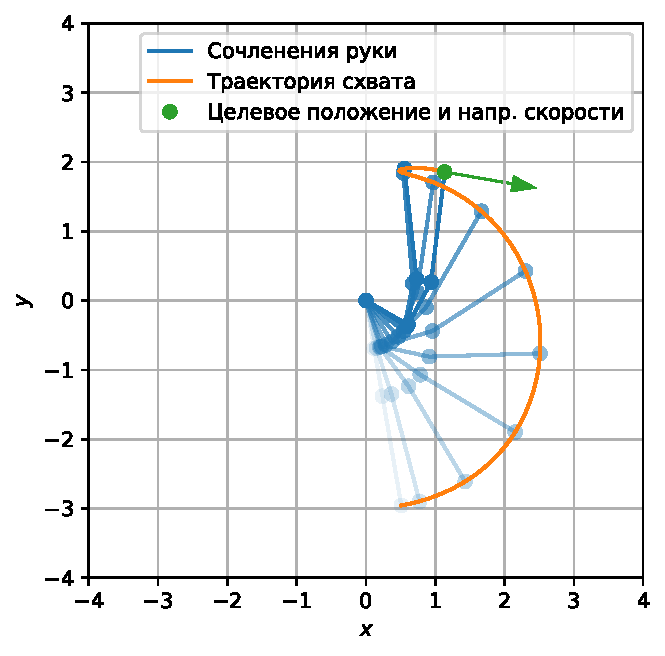
\includegraphics[width=0.49\textwidth]{examples/reaching_speed_pendulum}
            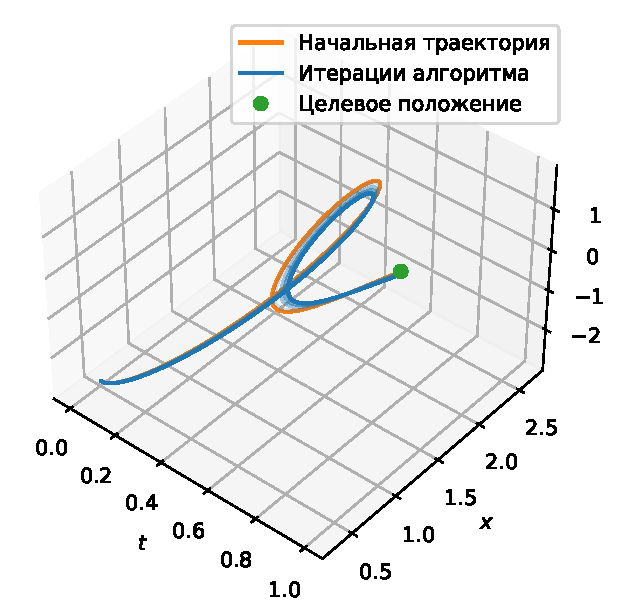
\includegraphics[width=0.49\textwidth]{examples/reaching_speed_endpoint}
        \end{center}
        \caption{Траектория системы при оптимальном управлении и итеративные траектории схвата для задачи целевого положения и скорости схвата. Алгоритм сошёлся на 7 итерации.}
        \label{fig:reaching-speed-task}
    \end{figure}

    \ifSubfilesClassLoaded{
        \nocite{*}
        \clearpage
        \bibliographystyle{plain}
        \bibliography{../../refs}
    }{}
\end{document}